\documentclass[letterpaper,11pt]{article}

\usepackage[utf8]{inputenc}
\usepackage{amsmath}
\usepackage{amsfonts}
\usepackage{amssymb}
\usepackage{amsthm}
\usepackage[spanish]{babel}
\usepackage{fontenc}
\usepackage{graphicx}
\graphicspath{ {./} }

\title{Fundamentos de Bases de Datos 2016-1\\Pŕactica 1}
\author{Jos\'e Ricardo Rodr\'{\i}guez Abreu \\ Ricardo Taboada Magallanes \\ Ricardo Jim\'enez M\'endez}
\date{\today\\ Facultad de Ciencias UNAM}

\begin{document}
 
 \maketitle

 \begin{center}
   {\bf 1. Ideas generales del proyecto:} 
 \end{center}
 La idea de crear y mantener una base de datos sobre una jugueter\'{\i}a, nace a partir de querer tener un orden respecto a los distintos procesos que podemos realizar en \'esta. \\
 La simple necesidad de conocer los productos que se venden hasta poder administrar los empleados, ingresos y egresos que se generan para mantener as\'{\i}, un balance respecto al capital. Los actores integrados en el servicio de venta de m\'ultiples productos y su distribuci\'on en m\'ultiples marcas y juguetes. Tambi\'en se puede implementar un sistema de compra diferente y eficiente al ser todo automatizado y garantizando su seguridad.

 \begin{center}
   {\bf 2. Listado de supusestos:}
 \end{center}
 
 \begin{enumerate}
 \item Poder ver y buscar que juguetes se venden.
 \item Realizar venta de jueguetes a usuarios.
 \item Realizar compra de jueguetes a distintos distribuidores de marcas como Mattel, Playmobile, etc.
 \item Tener informaci\'on sobre la disponibilidad de juguetes en distintas tiendas en tiempo real.
 \item Cotejar un balance sobre la cantidad ganada y gastada para obtener un intreso bruto de la suma del conjunto de todas las tiendas.
 \item Poder realizar altas/bajas de empleados, usuarios registrados y juguetes fuera de existencia.
 \item Modificar el precio de los productos de compra/venta. En especial el de los juguetes y el pago a empleados.
 \item Dar de alta/baja una nueva tienda.
 \item Poder sacar el monto total de pago para cada empleado dependiendo de su posici\'on, fecha de ingreso y ventas que ha hecho y cambiar de posici\'on a cada empleado cuando cumpla cierto tiempo.
 \item Tener un sistema de pedidos donde podamos ver el cliente, quien hizo la transacci\'on, el lugar en el que fue hecha y la fecha.
 \item As\'{\i} mismo poder obtener un pago automatizado con la tarjeta de cr\'edito del cliente para un proceso r\'apido.
 \item Dejar abierta la posibilidad de extenci\'on hacia un mercado online donde podamos hacer env\'{\i}os. 
 \end{enumerate}

 \begin{center}
   {\bf 3. Requerimientos candidatos: }
 \end{center}

 \begin{enumerate}
 \item Juguete\\
   Descripci\'on: Es el art\´{\i}culo principal de toda la tienda. Es lo que se va a vender y comprar. \\

   Valores:\\
   a) Estado: Aprovado. \\
   b) Costo: 2 semanas. \\
   c) Prioridad: Cr\'{\i}tico.\\
   d) Nivel de riezgo: Grave. \\
   \\
 \item Marca\\
   Descripci\'on: Cada uno de los jueguetes se clasifican a su vez por algunas marcas.\\

   Valores:\\
   a) Estado: Validado. \\
   b) Costo: 1 semana.\\
   c) Prioridad: Importante.\\
   d) Nivel de riezgo: Significativo.\\
   \\

   \item Distribuidor\\
   Descripci\'on: Es quien nos va a vender los juguetes a precio de mayoreo.\\

   Valores:\\
   a) Estado: Validado.\\
   b) Costo: 1 semana.\\
   c) Prioridad: Importante.\\
   d) Nivel de riezgo: Significativo.\\
   \\

   \item Sucursal\\
   Descripci\'on: Es el destino de los juguetes y es donde cada distribuidor llevar\'a los juguetes luego de ser comprados.\\

   Valores:\\
   a) Estado: Aprovado.\\
   b) Costo: 1 semana.\\
   c) Prioridad: Secundario.\\
   d) Nivel de riezgo: Medio.\\
   \\

   \item Empleado\\
   Descripci\'on: Es la persona que realiza las ventas en la tienda y tiene un costo elevado de p\'erdida. \\

   Valores:\\
   a) Estado: Aprovado.\\
   b) Costo: 3 d\'{\i}as.\\
   c) Prioridad: Secundario.\\
   d) Nivel de riezgo: Ordinario.\\
   \\

   \item Cliente\\
   Descripci\'on: Es el destino final de algunos de los juguetes. Es quien realiza las compras en tienda (posiblemente en l\'{\i}nea).\\

   Valores:\\
   a) Estado: Aprovado.\\
   b) Costo: 1 semana.\\
   c) Prioridad: Importante.\\
   d) Nivel de riezgo: Grave.\\
   \\

   \item Pedido\\
   Descripci\'on: Es el sistema que daremos para procesar una compra.\\

   Valores:\\
   a) Estado: Propuesto.\\
   b) Costo: 1 semana.\\
   c) Prioridad: Importante.\\
   d) Nivel de riezgo: Medio.\\
 \end{enumerate}


 \begin{center}
   {\bf 4. Requerimientos funcionales: }
 \end{center}
 \\
 a) Agregar y eliminar objetos:
 \begin{enumerate}
 \item Juguetes.
 \item Empleados.
 \item Sucursales.
 \item Clientes.
 \item Marcas.
 \item Distribuidores.
 \end{enumerate}
 b) Poder realizar el pago a los empleados. \\
 c) Optener ingresos. \\
 d) Realizar compra. \\ 

 

 \begin{center}
   {\bf 5. Requerimientos no funcionales no asociados: }
 \end{center}

 a) Poder ver fotos de los productos. \\
 b) Realizar un feedback del servicio. \\
 

 \begin{center}
   {\bf 6. Requerimientos no funcionales asociados: }
 \end{center}

 a) Promociones. \\
 
 \begin{center}
   {\bf 7. Diagrama de actividades: }
  
 \end{center}
 Adjunto a este archivo se envía el siguiente diagrama en formato .xml y .png.
 \\
 
  {\raggedleft{}  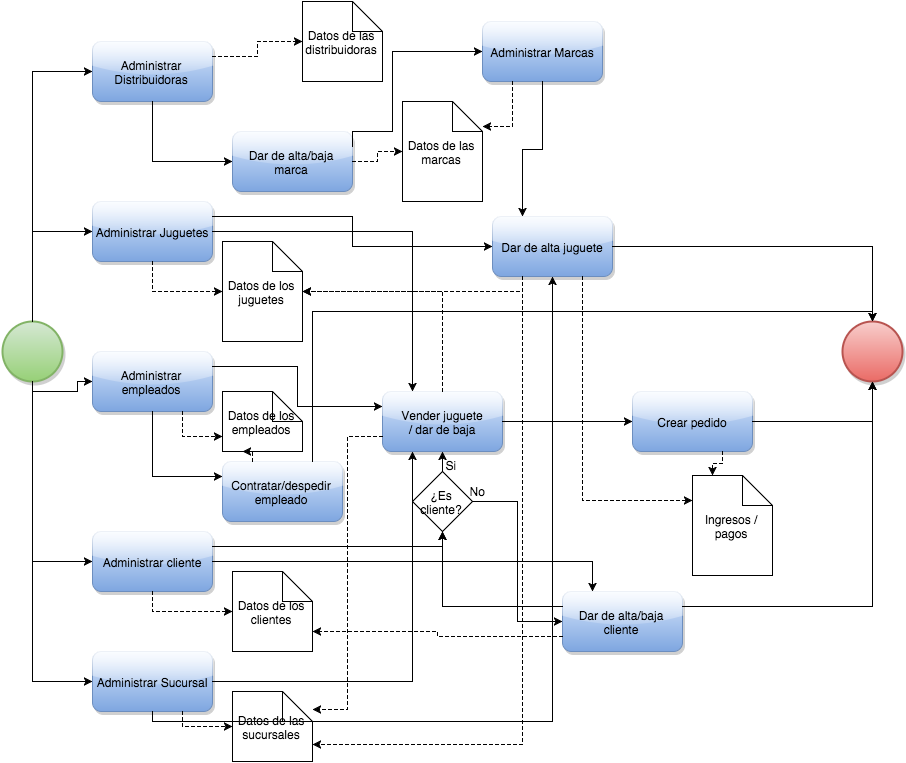
\includegraphics[width=10cm, height=10cm]{Diagrama_actividades} }
   
 \end{document}
